\documentclass[12pt]{article}
\usepackage{amsmath, amssymb, amsthm, graphicx}

\title{APPM 4600 \\ Homework 1}
\author{Dani Lisle | STID:109972839}
\date{\today}

\begin{document}
\maketitle

\newpage

% Problem 1
\section*{Problem 1}

Prompt: Plot the polynomial $p(x)$ and its expanded and factored forms. Explore the differences and their sources.

\subsubsection*{Parts i and ii}

The expanded form is shown in blue, and the factored form is shown in black.

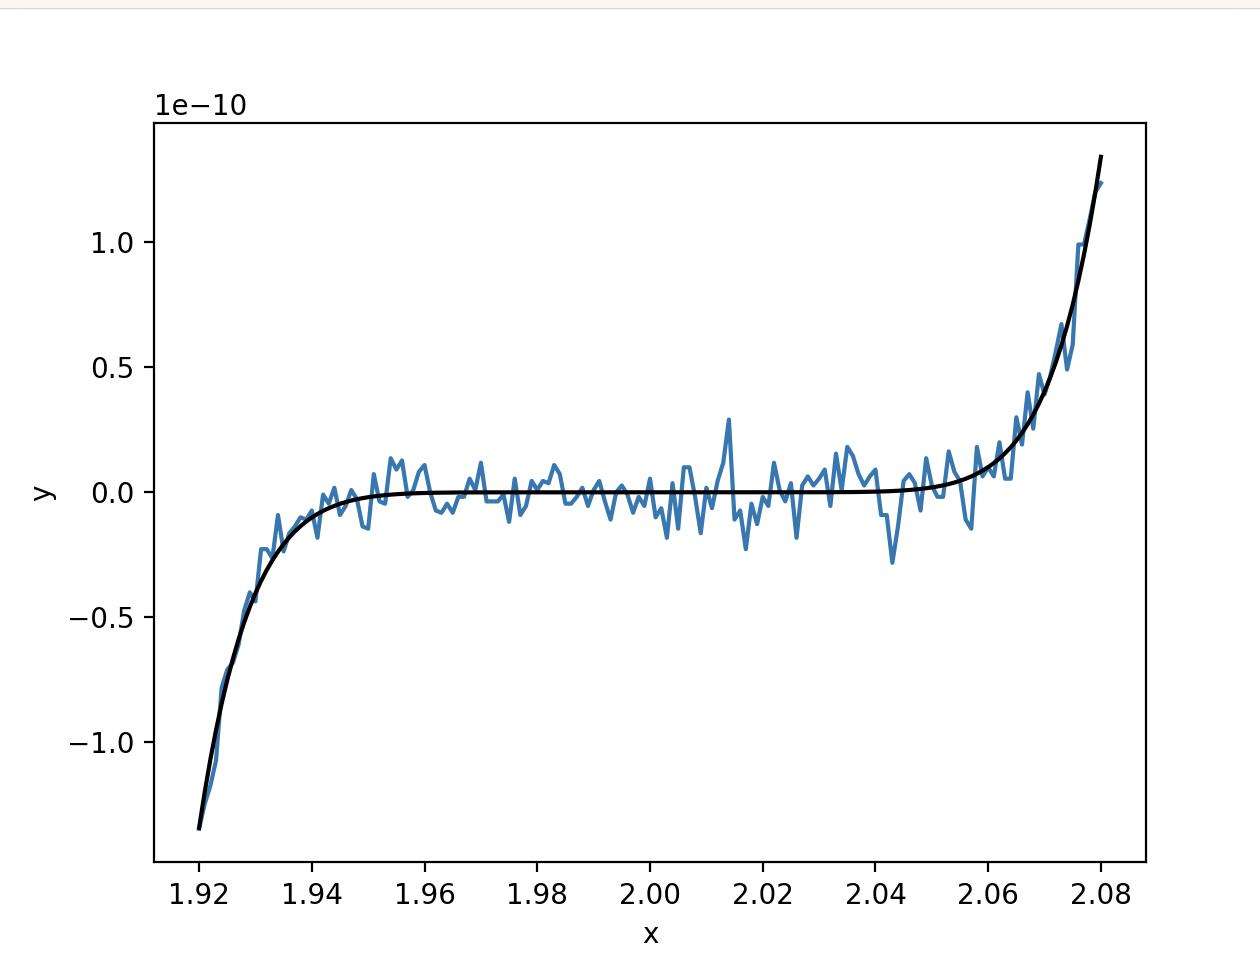
\includegraphics[width=\textwidth]{compare_polynomial_with_approx.png}


% List any assumptions for sub-problem 1.i here.
% Provide a detailed solution for sub-problem 1.i here.
% Discuss the solution for sub-problem 1.i here.


\subsubsection*{Part iii}

The black plot of the factored form is more correct. We know this based on our familiarity with functions of the form $(x-a)^b$. The blue plot of the expanded form has more numerical error from the addition of floating point numbers of various magnitudes, while the factored form avoids this.
% Problem 2
\section*{Problem 2}

Rewrite the expressions so they can be evaluated such as to avoid cancellation.

\subsubsection*{Part i}

Evaluate for x close to zero:

$$ \sqrt{x+1}-1 = \frac{(\sqrt{x+1}-1)(\sqrt{x+1}+1)}{(\sqrt{x+1}+1)} = \frac{x}{\sqrt{x+1}+1}

\subsubsection*{Part ii}

To evaluate for x close to y, use double-angle identities:

\begin{align*}
	\sin(x)-\sin(y) &= 2\cos(\frac{x+y}{2})\sin(\frac{x-y}{2}) \\
					&= 2\cos(\frac{x+y}{2})[\sin(x/2)\cos(-y/2)+\cos(x/2)\sin(-y/2)]
\end{align*}




\subsubsection*{Part iii}

Multiply and divide by the conjugate of the numerator:

\begin{align*}
	\frac{1-\cos x}{\sin x} &= \frac{(1-\cos x)(1+\cos x)}{\sin x(1+\cos x)}
							= \frac{1 - \cos^2 x}{\sin x + \sin x \cos x}
							= \frac{\sin^2 x}{\sin x + \sin x \cos x} \\
							&= \frac{\sin x}{1 + \cos x}
\end{align*}


\newpage

% Problem 3
\section*{Problem 3}

Find the second degree Taylor polynomial about 0 for $f(x) = (1+x+x^3)^3 \cos(x)$.

This is in the form

$$ P_2(x) = f(0) + f'(0)x + \frac{f''(0)}{2!}{x^2}  $$

We find the derivatives:

\begin{align*}
	f' &= (1+3x^2)\cos x - (1+x+x^3)\sin x \\
	f'' &= \cos x(5x - 1 - x^3) + \sin x(-2 - 6x^2)
\end{align*}

So, $	P_2(x) = 1 + x + x^2/2$.

\subsubsection*{Part a}

Approximate $f(0.5)$ using $P_2(0.5)$.

$$ P_x(0.5) = 1.3750... $$

Find an upper bound for the error $|f(0.5) - P_2(0.5)|$ and compare it to the actual error.

An upper bound for the error comes from the error term of the Taylor polynomial, and is expressed:

$$ \frac{|f'''(c)|}{3!}|0.5|^3 $$

where $ c$ is the value that maximizes $|f'''(c)|$ on the interval $[0,0.5]$.
Since $f'''(x) = (3-9x^2)\cos x + (1-17x+x^3) \sin x$, in this case $c = 0$, so the bound is

$$ \frac{3}{6}|0.5|^3 = 0.0625...$$

The actual error is 

$$|f(0.5)-P_2(0.5)| = |\frac{18}{8}\cos \frac{1}{2} - 1.3750| = 0.0510...$$

This is below the bound, as expected.

\subsubsection*{Part b}

Find a bound for $|f(x)-P_2(x)|$ for the approximation in general.

In general, the error when approximating $f$ at $x$ is bounded by

$$ \frac{|f'''(c)|}{3!}|x|^3 $$

where $ c$ is the value that maximizes $|f'''(c)|$ on the interval $[0,x]$.

\subsubsection*{Part c}

Approximate $\int_0^1 f(x) dx$ using $\int_0^1 P_2(x)dx$.

$$ \int_0^1 1+ x + \frac{x^2}{2} dx = x + x^2 + \frac{x^3}{3} |_0^1 = \frac{4}{3}

\subsubsection*{Part d}

Estimate the error in the integral.

We can estimate this without directly computing the true integral by using the error term again. Since integration is a linear operator, the error is bounded above by

$$ \int_0^1 \frac{|f'''(c)|}{3!}|x|^3 dx $$

where $ c$ maximizes $|f'''(c)|$ on $[0,x]$.

Since $c=0$ is the maximizer for all sub-intervals of $[0,1]$, this simplifies to 

$$ \frac{1}{2} \int_0^1 |x|^3 dx = \frac{1}{2} \frac{x^4}{4} |_0^1 = \frac{1}{8}

\newpage

% Problem 4
\section*{Problem 4}

Consider $x^2 - 56x + 1$.

\subsubsection*{Part a}

Compute the relative errors for the two roots using the quadratic formula, assuming you can calculate the square root to 3 significant digits.

The absolute error for both is $\pm \frac{1}{4}10^{-3}$. Using the formula we find the roots are $28 \pm 3 \sqrt 87$. We can compute these are approximately 0.0178628 and 55.9821.

Using 

$$\text{Relative Error} = \frac{\text{Approximate}}{\text{Actual}}

we find the relative errors are about 0.014 and 4.47e-6, respectively.

\subsubsection*{Part b}

The "bad" root is $28 - 3\sqrt87$, corresponding to 

$$ x = \frac{-b - \sqrt{b^2 - 4ac}}{2a} $$

We multiply and divide by the conjugate of the numerator:

\begin{align*}
	x &= \frac{(-b - \sqrt{b^2 - 4ac})(-b + \sqrt{b^2 - 4ac})}{2a(-b + \sqrt{b^2 - 4ac})} \\
	&= \frac{(-b)^2 - (\sqrt{b^2 - 4ac})^2}{2a(-b + \sqrt{b^2 - 4ac})} \\
	&= \frac{2c}{-b + \sqrt{b^2 - 4ac}}
\end{align*}

This algorithm allows us to calculate the smaller root with more lower relative error.


% Problem 5
\section*{Problem 5}
\subsubsection*{Part a}

Find upper bounds on the error $|\Delta y|$ and the relative error  $|\Dedlta y|/|y|$ and find when the relative error is large.

When $x_1$ is large and $x_2$ is small, the absolute error is bounded by $|\Delta x_1 - \Delta x_2|$ and the relative error is bounded by 

$$ \frac{|\Delta x_1 - \Delta x_2|}{|x_1-x_2|}$$

\subsubsection*{Part b}

Using the sum-to-sum product identities, we can manipulate $\cos(x + \delta) - \cos(x) $ into

$$-2 \sin\left(x + \frac{\delta}{2}\right) \sin\left(\frac{\delta}{2}\right) $$


\end{document}